% inkscape koch-rule.pdf --export-type=png --export-filename=koch-rule.png --export-width=1024 --export-background-opacity=0
% \documentclass[a3paper]{article}
% \usepackage[left=0mm,top=1cm,right=0mm,bottom=0mm]{geometry}
\documentclass[border=0]{standalone}
% \documentclass[dvisvgm]{minimal}
\usepackage{tikz}
\usetikzlibrary{calc,lindenmayersystems}
\usepackage{xcolor}
\definecolor{pGreen}{HTML}{663366}
\definecolor{pRed}{HTML}{336633}
\pgfdeclarelindenmayersystem{Koch curve}{\rule{F -> F+F--F+F}}
\begin{document}
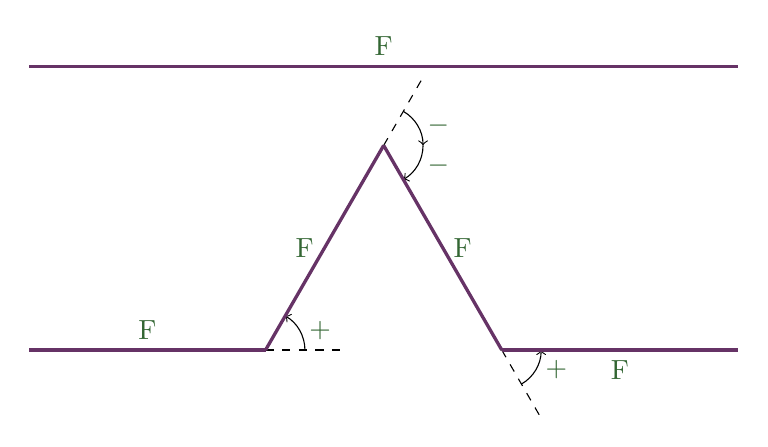
\begin{tikzpicture}
      \pgfmathsetmacro{\g}{1+3*sqrt(3)/2}
      \draw[very thick, pGreen,yshift=\g cm] (0,0) -- node[midway,above,pRed] {F} (9,0);
      \draw[very thick, pGreen] (0,0) -- node[midway,above,pRed] {F} (3,0);
      \draw[thin,dashed] (3,0) -- ++(0:1);
      \draw[->] (3.5,0) arc [start angle=0, end angle=60, radius=5mm] node[midway,right,pRed] {$+$};
      \draw[very thick, pGreen] (3,0) --++ (60:3) node[midway,left,pRed] {F};
      \draw[thin,dashed] (3,0)++(60:3) --++ (60:1);
      \draw[->] (3,0)++(60:3.5) arc [start angle=60, end angle=0, radius=5mm] node[midway,right,pRed] {$-$};
      \draw[->] ($ (3,0)+(60:3)+(0:0.5) $) arc [start angle=0, end angle=-60, radius=5mm] node[midway,right,pRed] {$-$};
      \draw[very thick, pGreen] ($(3,0)+(60:3)$) --++ (-60:3) node[midway,right,pRed] {F};
      \draw[thin,dashed] (6,0) --++ (-60:1);
      \draw[->] ($ (6,0)+(-60:0.5)$) arc [start angle=-60, end angle=0, radius=5mm] node[midway,right,pRed] {$+$};
      \draw[very thick, pGreen] (6,0) -- (9,0) node[midway,below,pRed] {F};
      % \draw [pGreen,line width=7pt] [l-system={Koch curve, step=20, angle=60, axiom=F, order=6}] lindenmayer system;
\end{tikzpicture}
\end{document}